% ============================================================
%  SolarIntel — Academic Research Paper
%  "SolarIntel: Machine Learning and Agentic AI for Solar
%   Energy Forecasting and Grid Optimisation Across
%   European Markets"
%  Author: Mahir
% ============================================================
\documentclass[11pt]{article}

% ---- Packages -----------------------------------------------
\usepackage[top=2cm,bottom=2cm,left=1.8cm,right=1.8cm]{geometry}
\usepackage{newtxtext,newtxmath}
\usepackage{amsmath}
\usepackage{graphicx}
\usepackage{booktabs}
\usepackage{tabularx}
\usepackage[hidelinks,colorlinks=true,linkcolor=navyblue,citecolor=navyblue,urlcolor=navyblue]{hyperref}
\usepackage{tikz}
\usetikzlibrary{shapes.geometric,arrows.meta,positioning,fit,backgrounds,calc}
\usepackage{float}
\usepackage{caption}
\usepackage{multicol}
\usepackage{abstract}
\usepackage{fancyhdr}
\usepackage[explicit]{titlesec}
\usepackage{xcolor}
\usepackage{enumitem}
\usepackage{microtype}
\usepackage{parskip}
\usepackage{setspace}
\usepackage[htt]{hyphenat}
\usepackage{url}
\def\UrlBreaks{\do\_\do\.\do\-\do\/\do\~}
\emergencystretch=4em
\hyphenpenalty=50
\exhyphenpenalty=50

% ---- Colours (matching detailed report palette) -------------
\definecolor{solarblue}{RGB}{31,78,121}
\definecolor{solaramber}{RGB}{180,100,20}
\definecolor{solargray}{RGB}{80,80,80}
\definecolor{navyblue}{RGB}{31,78,121}   % alias for compatibility
\definecolor{lightnavy}{RGB}{220,228,245}

% ---- Section heading style ----------------------------------
\titleformat{\section}
  {\normalfont\bfseries\color{solarblue}}
  {\thesection.}{0.5em}{#1}[\color{solarblue}\titlerule]

\titleformat{\subsection}
  {\normalfont\bfseries\color{solaramber}}
  {\thesubsection}{0.5em}{#1}

\titleformat{\subsubsection}
  {\normalfont\itshape\color{solargray}}
  {\thesubsubsection}{0.5em}{#1}

\titlespacing*{\section}{0pt}{10pt}{5pt}
\titlespacing*{\subsection}{0pt}{8pt}{4pt}
\titlespacing*{\subsubsection}{0pt}{6pt}{3pt}

% ---- Header / footer ----------------------------------------
\pagestyle{fancy}
\fancyhf{}
\renewcommand{\headrulewidth}{0.4pt}
\fancyhead[L]{\small\color{solarblue}\textit{SolarIntel: ML and Agentic AI for Solar Energy Forecasting}}
\fancyhead[R]{\small\color{solarblue}\textit{Solar Energy Generation Prediction}}
\fancyfoot[C]{\small\thepage}

% ---- Abstract package tweak (single-col abstract) -----------
\renewcommand{\abstractnamefont}{\normalfont\large\bfseries\color{solarblue}}
\renewcommand{\abstracttextfont}{\normalfont\normalsize}
\setlength{\absleftindent}{0pt}
\setlength{\absrightindent}{0pt}
\setlength{\abstitleskip}{8pt}

% ---- Caption style ------------------------------------------
\captionsetup{font=small,labelfont={bf,color=solarblue},skip=6pt}

% ---- Column separation --------------------------------------
\setlength{\columnsep}{20pt}

% ---- Line spacing -------------------------------------------
\setstretch{1.08}

% ---- Paragraph spacing --------------------------------------
\setlength{\parskip}{4pt}

% ---- List style ---------------------------------------------
\setlist[itemize]{leftmargin=*,itemsep=3pt,topsep=4pt}
\setlist[enumerate]{leftmargin=*,itemsep=3pt,topsep=4pt}

% =============================================================
\begin{document}

% ---- Title block (full width, before multicols) -------------

  \begin{center}
    {\fontsize{22}{26}\bfseries\color{solarblue} SolarIntel}\\[8pt]
    {\large\color{solaramber} Machine Learning and Agentic AI for Solar Energy Forecasting\\[3pt] and Grid Optimisation Across European Markets}\\[20pt]
  \end{center}

  \vspace{6pt}
  \begin{abstract}
    \vspace{6pt}
    \noindent
    Accurate solar energy forecasting and actionable grid advisory are essential
    for integrating variable renewable generation into modern power systems.
    This paper presents \textit{SolarIntel}, a two-phase end-to-end system that
    addresses both challenges at European scale. In Phase~1, a machine learning
    pipeline fuses the EMHIRES solar capacity factor dataset (29 countries,
    1986--2015, hourly) with NASA POWER meteorological reanalysis data
    (2001--2015), yielding a merged corpus of approximately 3.8~million records
    across 34 engineered features. A Random Forest Regressor achieves
    \(R^2 = 0.9112\), MAE = 0.0280, and RMSE = 0.0547 on the held-out test set,
    outperforming a Linear Regression baseline (\(R^2 = 0.7880\)) by a substantial
    margin. In Phase~2, a LangGraph-based agentic pipeline augments these
    forecasts with deterministic risk analysis, retrieval-augmented generation
    (RAG) over a curated energy knowledge base, and structured LLM reasoning to
    produce JSON-formatted grid management recommendations. Together, the two
    phases demonstrate a scalable, reproducible pathway from raw meteorological
    inputs to operational decision support across diverse European grid contexts.
  \end{abstract}
  \vspace{6pt}

  \vspace{4pt}
  \noindent\textbf{Keywords:} solar energy forecasting, random forest regression,
  LangGraph, retrieval-augmented generation, grid advisory, EMHIRES, NASA POWER,
  agentic AI, European energy systems\\[20pt]

% =============================================================
\begin{multicols}{2}
\section{Introduction}
% =============================================================

The decarbonisation of European electricity grids has accelerated the deployment
of photovoltaic (PV) capacity across the continent, with aggregate installed
capacity exceeding 260~GW by 2023~\cite{irena2023}. Unlike dispatchable
generation, solar PV output is governed by meteorological conditions that vary
on sub-hourly timescales, imposing forecasting and balancing challenges on
transmission and distribution system operators. Accurate short-term and
day-ahead forecasts reduce reserve requirements, lower balancing costs, and
enable efficient intraday market participation~\cite{antonanzas2016}.

Despite a rich literature on data-driven solar forecasting, two gaps remain.
First, most published models are trained on single-site or single-country data,
limiting their geographic transferability. Second, forecast outputs are rarely
connected to actionable grid management guidance; operators must translate
numerical predictions into operational decisions without systematic support.

\textit{SolarIntel} addresses both gaps. Phase~1 trains machine learning models
on a pan-European dataset covering 29 countries and 15 years, producing
capacity factor predictions with high accuracy. Phase~2 wraps these predictions
in a four-node agentic pipeline that performs risk analysis, retrieves relevant
domain knowledge, and generates structured, auditable recommendations via a
large language model (LLM).

The remainder of this paper is organised as follows. Section~2 surveys related
work. Section~3 describes dataset construction and feature engineering.
Section~4 details the ML models. Section~5 presents the agentic architecture.
Sections~6 and~7 cover the RAG pipeline and LLM integration respectively.
Section~8 reports results and evaluation. Sections~9 and~10 discuss limitations
and conclude.

% =============================================================
\section{Related Work}
% =============================================================

\subsection{Machine Learning for Solar Forecasting}

Data-driven solar forecasting has evolved from autoregressive statistical
methods towards ensemble and deep learning approaches. Voyant et al.\ provide
a comprehensive survey of machine learning methods applied to solar radiation
and PV output forecasting, documenting consistent improvements of ensemble
methods over linear baselines~\cite{voyant2017}. Breiman's Random Forest
algorithm~\cite{breiman2001} has been widely adopted in this domain due to its
robustness to feature collinearity, resistance to overfitting via bagging, and
interpretability through feature importance scores. Antonanzas et al.\ review
post-processing and spatial ensemble strategies for PV power forecasting,
highlighting the value of large-scale, multi-site training corpora~\cite{antonanzas2016}.

\subsection{Retrieval-Augmented Generation in Energy Systems}

Lewis et al.\ introduced retrieval-augmented generation (RAG) as a method for
grounding LLM outputs in external, verifiable knowledge, demonstrating reduced
hallucination and improved factual accuracy~\cite{lewis2020}. Subsequent work
has applied RAG principles to domain-specific question answering in technical
and scientific fields. The energy sector presents a compelling use case: grid
operation involves large, evolving corpora of standards, market rules, and
operational guidelines that cannot be fully internalised by a pretrained LLM.

\subsection{Agentic and Multi-Agent AI Pipelines}

The emergence of LangGraph~\cite{langchain2024} and similar graph-based
orchestration frameworks has enabled the construction of stateful, multi-node
AI pipelines in which different nodes perform specialised tasks---forecasting,
retrieval, reasoning---and communicate via a shared typed state. This paradigm
extends single-LLM chat interfaces to structured decision workflows with
deterministic intermediate steps, improving auditability and enabling modular
testing of individual components.

% =============================================================
\section{Dataset and Feature Engineering}
% =============================================================

\subsection{EMHIRES Solar Dataset}

The European Meteorological derived HIgh REsolution RES generation time series
(EMHIRES) dataset, published by the Joint Research Centre of the European
Commission~\cite{gonzalez2016}, provides hourly solar capacity factors for
29~European countries spanning 1986--2015 in wide format, with one column per
country and one row per hour. A capacity factor represents the ratio of actual
to rated power output and lies on the unit interval \([0, 1]\). The dataset
contains approximately \(262{,}800\) hourly timestamps at full European coverage.

\textbf{Reshape to long format.} The wide-format EMHIRES table is melted via
\texttt{pandas.DataFrame.melt} to produce a long-format table with three
columns: \texttt{Timestamp}, \texttt{Country}, and \texttt{Capacity\_Factor}.
This transformation is implemented in
\texttt{Final\_Pipeline/Final\_Pipeline.py} and yields approximately
\(7.6\)~million rows prior to temporal filtering.

\subsection{NASA POWER Meteorological Data}

The NASA Prediction of Worldwide Energy Resources (POWER) project~\cite{stackhouse2019}
provides gridded reanalysis meteorological parameters derived from satellite
observations and atmospheric models. For each of the 29~country centroids,
three hourly parameters are retrieved for the period 2001--2015 via the NASA
POWER REST API (implemented in \texttt{NASA\_Data\_Fetch/fetcher.py}):

\begin{itemize}
  \item \textbf{Irradiance} (\texttt{ALLSKY\_SFC\_SW\_DWN}): all-sky surface
        shortwave downwelling irradiance, W/m$^2$.
  \item \textbf{Temperature} (\texttt{T2M}): air temperature at 2~m height, $^\circ$C.
  \item \textbf{Wind\_Speed} (\texttt{WS10M}): wind speed at 10~m height, m/s.
\end{itemize}

Missing-value sentinel handling is a critical preprocessing step: NASA POWER
encodes missing observations as \(-999.0\). All rows where any meteorological
parameter equals \(-999.0\) are dropped prior to merging, as implemented in the
cleaning stage of \texttt{Final\_Pipeline/Final\_Pipeline.py}.

\subsection{Dataset Merge and Temporal Alignment}

EMHIRES timestamps begin at \texttt{1986-01-01 00:00:00} with hourly frequency.
Since NASA POWER data is available from 2001, the merged dataset covers
2001--2015 (15~years), corresponding to \(131{,}400\) hourly timestamps per
country. After an inner join on \texttt{(Timestamp, Country)}, dropping
\(-999\)-flagged rows and rows with any remaining \texttt{NaN} values, the
cleaned corpus contains approximately \textbf{3.8~million rows}. The merge is
executed in \texttt{Final\_Pipeline/Final\_Pipeline.py} using
\texttt{pandas.merge} on the composite key.

\subsection{Feature Engineering}

Two temporal features are extracted from the \texttt{Timestamp} column:
\texttt{Hour} (integer, 0--23) and \texttt{Month} (integer, 1--12). These
capture the diurnal solar cycle and seasonal variation respectively without
requiring cyclic encoding, as tree-based models can partition on these ordinal
values directly.

Geographic variation across the 29 countries is encoded via one-hot encoding
of the \texttt{Country} column, producing 29 binary indicator columns
(\texttt{Country\_AT} through \texttt{Country\_UK}). The complete feature
matrix therefore contains \textbf{34 columns}: 5 continuous features
(\texttt{Hour}, \texttt{Month}, \texttt{Irradiance}, \texttt{Temperature},
\texttt{Wind\_Speed}) plus 29 country indicator columns. The target variable
is \texttt{Capacity\_Factor} $\in [0, 1]$.

\subsection{Train/Test Split}

The dataset is partitioned into training (80\%) and test (20\%) subsets using
\path{sklearn.model_selection.train_test_split} with \texttt{random\_state=67},
yielding approximately 3.05~million training rows and 763~thousand test rows.
The split is random across all timestamps and countries, which tests
interpolation within the observed distribution rather than temporal
extrapolation.

Figure~\ref{fig:pipeline} illustrates the complete Phase~1 data and model pipeline.

\end{multicols}
\begin{figure}[H]
\centering
\resizebox{0.52\textwidth}{!}{%
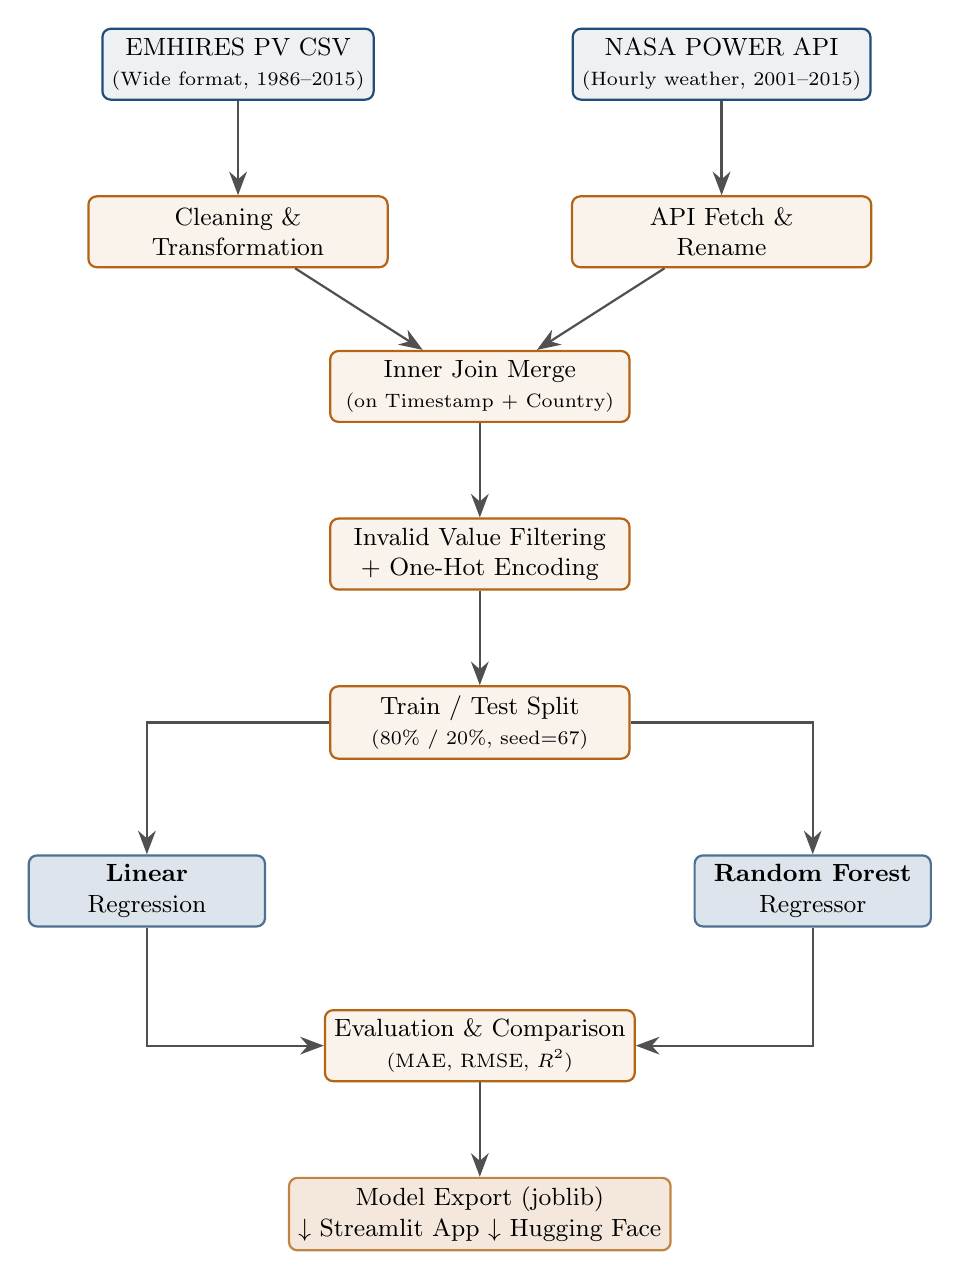
\begin{tikzpicture}[
    node distance=1.2cm and 2.5cm,
    every node/.style={font=\small},
    databox/.style={rectangle, draw=solarblue, fill=solarblue!8, rounded corners=3pt, minimum width=3.2cm, minimum height=0.9cm, align=center, thick},
    procbox/.style={rectangle, draw=solaramber, fill=solaramber!8, rounded corners=3pt, minimum width=3.8cm, minimum height=0.9cm, align=center, thick},
    modelbox/.style={rectangle, draw=solarblue!80, fill=solarblue!15, rounded corners=3pt, minimum width=3cm, minimum height=0.9cm, align=center, thick},
    deploybox/.style={rectangle, draw=solaramber!80, fill=solaramber!15, rounded corners=3pt, minimum width=4cm, minimum height=0.9cm, align=center, thick},
    arrow/.style={-{Stealth[length=3mm]}, thick, color=solargray}
]
\node[databox] (emhires) {EMHIRES PV CSV\\{\scriptsize (Wide format, 1986--2015)}};
\node[databox, right=of emhires] (nasa) {NASA POWER API\\{\scriptsize (Hourly weather, 2001--2015)}};
\node[procbox, below=of emhires] (clean) {Cleaning \&\\Transformation};
\node[procbox, below=of nasa] (fetch) {API Fetch \&\\Rename};
\node[procbox, below=1.5cm of $(clean)!0.5!(fetch)$] (merge) {Inner Join Merge\\{\scriptsize (on Timestamp + Country)}};
\node[procbox, below=of merge] (filter) {Invalid Value Filtering\\+ One-Hot Encoding};
\node[procbox, below=of filter] (split) {Train / Test Split\\{\scriptsize (80\% / 20\%, seed=67)}};
\node[modelbox, below left=1.2cm and 0.8cm of split] (lr) {\textbf{Linear}\\Regression};
\node[modelbox, below right=1.2cm and 0.8cm of split] (rfr) {\textbf{Random Forest}\\Regressor};
\node[procbox, below=1.5cm of $(lr)!0.5!(rfr)$] (eval) {Evaluation \& Comparison\\{\scriptsize (MAE, RMSE, $R^2$)}};
\node[deploybox, below=of eval] (deploy) {Model Export (joblib)\\$\downarrow$ Streamlit App $\downarrow$ Hugging Face};
\draw[arrow] (emhires) -- (clean);
\draw[arrow] (nasa) -- (fetch);
\draw[arrow] (clean) -- (merge);
\draw[arrow] (fetch) -- (merge);
\draw[arrow] (merge) -- (filter);
\draw[arrow] (filter) -- (split);
\draw[arrow] (split) -| (lr);
\draw[arrow] (split) -| (rfr);
\draw[arrow] (lr) |- (eval);
\draw[arrow] (rfr) |- (eval);
\draw[arrow] (eval) -- (deploy);
\end{tikzpicture}%
}
\caption{SolarIntel Phase~1 pipeline architecture.}
\label{fig:pipeline}
\end{figure}

\newpage
\begin{multicols}{2}

% =============================================================
\section{Machine Learning Models}
% =============================================================

\subsection{Linear Regression Baseline}

An ordinary least-squares linear regression model is trained as a baseline to
quantify the marginal benefit of the ensemble approach. The model is
implemented via \path{sklearn.linear_model.LinearRegression} with default
hyperparameters and fits a 34-dimensional hyperplane to the training data.
Its closed-form solution is unique and computationally tractable at the
3.8~million row scale. Linear regression serves as an interpretability anchor:
its coefficients reveal the direction and magnitude of each feature's marginal
contribution, modulo the assumption of additive independence.

\subsection{Random Forest Regressor}

The primary predictive model is a
\path{sklearn.ensemble.RandomForestRegressor} configured with the following
hyperparameters:

\begin{itemize}
  \item \texttt{n\_estimators = 100}: 100 decision tree base learners.
  \item \texttt{max\_depth = 12}: maximum tree depth, balancing expressiveness
        against overfitting.
  \item \texttt{random\_state = 67}: controls bootstrap sampling and feature
        subsampling for reproducibility.
\end{itemize}

At each internal node, the algorithm evaluates a random subset of
\(\sqrt{34} \approx 6\)~features and selects the split that minimises the
mean squared error of the two resulting child nodes. Bootstrap aggregation
over 100 trees reduces variance relative to any single tree. The trained
models are serialised via \texttt{joblib} and archived in
\texttt{Models/solar\_models.zip} as \texttt{solar\_model\_lr.pkl} and
\texttt{solar\_model\_rfr.pkl}.

\subsection{Evaluation Metrics}

Model performance is assessed on the held-out test set using three standard
regression metrics. The coefficient of determination $R^2$ quantifies the
proportion of variance explained:
\[
  R^2 = 1 - \frac{\displaystyle\sum_{i}(y_i - \hat{y}_i)^2}
                  {\displaystyle\sum_{i}(y_i - \bar{y})^2}
\]
Mean Absolute Error (MAE) measures average absolute deviation in capacity
factor units, and Root Mean Squared Error (RMSE) penalises large errors more
heavily. Both are expressed in dimensionless capacity factor units. The
complete evaluation pipeline is implemented in
\texttt{Final\_Pipeline/Final\_Pipeline.py}.

\begin{table}[H]
  \centering
  \caption{Model performance on the held-out test set (20\% random split).}
  \label{tab:model_metrics}
  \small
  \begin{tabular}{lccc}
    \toprule
    \textbf{Model} & $\boldsymbol{R^2}$ & \textbf{MAE} & \textbf{RMSE} \\
    \midrule
    Linear Regression  & 0.7880 & 0.0534 & 0.0845 \\
    Random Forest      & \textbf{0.9112} & \textbf{0.0280} & \textbf{0.0547} \\
    \bottomrule
  \end{tabular}
\end{table}

The Random Forest achieves a 12.3 percentage point improvement in $R^2$,
a 47.6\% reduction in MAE, and a 35.3\% reduction in RMSE relative to the
linear baseline, confirming that the relationship between the feature set and
capacity factor is substantially non-linear. The RMSE improvement is
particularly meaningful for grid operators because large prediction errors at
peak or near-zero output periods carry asymmetric operational costs.

% =============================================================
\section{Agentic AI Architecture}
% =============================================================

\subsection{Design Rationale}

Pure ML forecasting models produce numerical capacity factor estimates but do
not themselves generate actionable operational guidance. Bridging the gap
between a predicted 24-hour profile and concrete grid management actions
requires domain knowledge about battery energy storage system (BESS) dispatch
strategies, demand-side management (DSM), intraday market mechanisms, and
balancing reserve obligations. Rather than hard-coding this knowledge in
procedural rules, Phase~2 of SolarIntel implements a composable agentic
pipeline in which specialised nodes perform retrieval and reasoning over a
curated knowledge base.

\subsection{LangGraph StateGraph}

The Phase~2 pipeline is implemented as a \texttt{StateGraph} using the
LangGraph framework~\cite{langchain2024}, which models the pipeline as a
directed acyclic graph (DAG) of nodes connected by typed edges. The graph is
defined in \texttt{Agent\_Pipeline/graph.py}. Execution proceeds
deterministically from the \texttt{forecast\_node} through the
\texttt{risk\_node}, \texttt{rag\_node}, and \texttt{recommend\_node} in
sequence, with no conditional branching or cycles. This linear topology
reflects the strict data dependency between stages: each node's output is a
necessary input to the next.

\subsection{Shared State: \texttt{GridAdvisorState}}

All inter-node communication occurs through a single shared state object,
\texttt{GridAdvisorState}, defined as a \texttt{TypedDict} in
\texttt{Agent\_Pipeline/state.py}. The state carries the following fields as
it propagates through the graph:

\begin{itemize}
  \item \texttt{country}, \texttt{capacity\_kw}, \texttt{date}: user-supplied
        input parameters.
  \item \texttt{weather\_data}: raw 24-hour meteorological forecast from
        Open-Meteo.
  \item \texttt{hourly\_cf}: list of 24 predicted capacity factor values from
        the RFR model.
  \item \texttt{risk\_flags}: structured output of the risk analysis node,
        including the variability score and ramp event list.
  \item \texttt{rag\_context}: concatenated text chunks retrieved from
        ChromaDB.
  \item \texttt{recommendations}: final JSON object from the LLM node.
\end{itemize}

Using a typed dictionary for shared state enforces a clear data contract
between nodes and simplifies debugging, since each node's input and output
can be inspected independently without access to adjacent nodes.

\subsection{Pipeline Architecture}

Figure~\ref{fig:architecture} illustrates the four-node pipeline and the
\texttt{GridAdvisorState} shared bus.

\end{multicols}
\begin{figure}[H]
\centering
\resizebox{0.72\textwidth}{!}{%
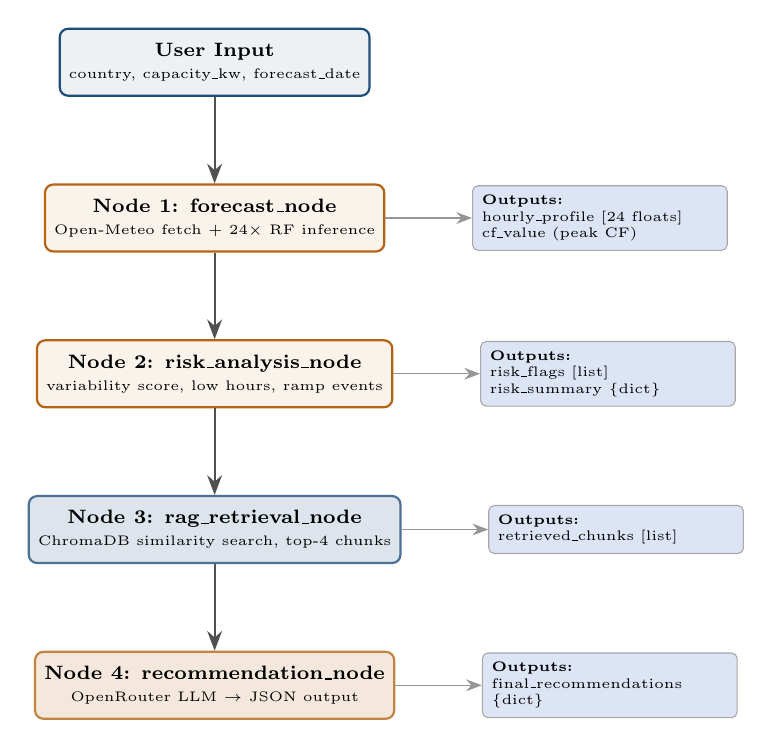
\begin{tikzpicture}[
    node distance=1.1cm,
    every node/.style={font=\scriptsize},
    databox/.style={rectangle, draw=solarblue, fill=solarblue!8, rounded corners=3pt,
                    minimum width=3.8cm, minimum height=0.85cm, align=center, thick},
    procbox/.style={rectangle, draw=solaramber, fill=solaramber!8, rounded corners=3pt,
                    minimum width=3.8cm, minimum height=0.85cm, align=center, thick},
    modelbox/.style={rectangle, draw=solarblue!80, fill=solarblue!15, rounded corners=3pt,
                     minimum width=3.8cm, minimum height=0.85cm, align=center, thick},
    deploybox/.style={rectangle, draw=solaramber!80, fill=solaramber!15, rounded corners=3pt,
                      minimum width=3.8cm, minimum height=0.85cm, align=center, thick},
    sidenote/.style={rectangle, draw=solargray!50, fill=lightnavy, rounded corners=2pt,
                     minimum width=3.0cm, align=left, font=\tiny, text width=3.0cm},
    arrow/.style={-{Stealth[length=2.5mm]}, thick, color=solargray},
    sidearrow/.style={-{Stealth[length=2mm]}, thin, color=solargray!60}
]
\node[databox] (input) {\textbf{User Input}\\{\tiny country, capacity\_kw, forecast\_date}};
\node[procbox, below=of input] (n1) {\textbf{Node 1: forecast\_node}\\{\tiny Open-Meteo fetch + 24$\times$ RF inference}};
\node[procbox, below=of n1] (n2) {\textbf{Node 2: risk\_analysis\_node}\\{\tiny variability score, low hours, ramp events}};
\node[modelbox, below=of n2] (n3) {\textbf{Node 3: rag\_retrieval\_node}\\{\tiny ChromaDB similarity search, top-4 chunks}};
\node[deploybox, below=of n3] (n4) {\textbf{Node 4: recommendation\_node}\\{\tiny OpenRouter LLM $\rightarrow$ JSON output}};
\node[sidenote, right=1.1cm of n1] (sn1)
    {\textbf{Outputs:}\\hourly\_profile [24 floats]\\cf\_value (peak CF)};
\node[sidenote, right=1.1cm of n2] (sn2)
    {\textbf{Outputs:}\\risk\_flags [list]\\risk\_summary \{dict\}};
\node[sidenote, right=1.1cm of n3] (sn3)
    {\textbf{Outputs:}\\retrieved\_chunks [list]};
\node[sidenote, right=1.1cm of n4] (sn4)
    {\textbf{Outputs:}\\final\_recommendations \{dict\}};
\draw[arrow] (input) -- (n1);
\draw[arrow] (n1) -- (n2);
\draw[arrow] (n2) -- (n3);
\draw[arrow] (n3) -- (n4);
\draw[sidearrow] (n1.east) -- (sn1.west);
\draw[sidearrow] (n2.east) -- (sn2.west);
\draw[sidearrow] (n3.east) -- (sn3.west);
\draw[sidearrow] (n4.east) -- (sn4.west);
\end{tikzpicture}%
}
\caption{Grid Advisor LangGraph pipeline: four sequential nodes with state outputs annotated.}
\label{fig:architecture}
\end{figure}
\begin{multicols}{2}

\subsection{Node 1: Forecast Node}

The Forecast Node (\texttt{Agent\_Pipeline/1\_forecast/node.py}) performs two
operations. First, it queries the Open-Meteo REST API~\cite{openmeteo2023} to
retrieve a 24-hour ahead hourly forecast for the target country's geographic
centroid, obtaining irradiance, 2~m temperature, and 10~m wind speed.
Open-Meteo is selected for its free, unauthenticated, production-grade
meteorological forecasts derived from ECMWF and other numerical weather
prediction models. Second, for each of the 24 hours, the node constructs a
34-dimensional feature vector---incorporating the hour index, current month,
retrieved weather parameters, and the appropriate one-hot country
indicator---and passes it to the pre-loaded Random Forest Regressor. The
result is a list of 24 capacity factor values stored in
\texttt{GridAdvisorState[``hourly\_cf'']}.

\subsection{Node 2: Risk Analysis Node}

The Risk Analysis Node (\texttt{Agent\_Pipeline/2\_risk/node.py}) applies
deterministic analytical rules to the 24-hour capacity factor profile. Three
risk signals are computed:

\begin{enumerate}
  \item \textbf{Variability score} $V$: the normalised mean absolute ramp rate
        (defined formally in Section~8.2), quantifying intra-day generation
        smoothness.
  \item \textbf{Low-output hours}: hours where the predicted capacity factor
        falls below 10\% of the daily peak, indicating periods of negligible
        generation that may require backup dispatch.
  \item \textbf{Ramp events}: consecutive-hour transitions where the absolute
        change in capacity factor exceeds 0.12, i.e.\
        $|\mathrm{CF}_h - \mathrm{CF}_{h-1}| > 0.12$, representing rapid
        generation changes that stress frequency regulation reserves.
\end{enumerate}

All three signals are computed without any LLM invocations, ensuring
determinism and low latency. Results are stored in
\texttt{GridAdvisorState[``risk\_flags'']}.

\subsection{Node 3: RAG Retrieval Node}

The RAG Retrieval Node (\texttt{Agent\_Pipeline/3\_rag/node.py}) retrieves
domain-relevant text passages from an in-memory vector store given the current
risk profile. The design and operation of this node are detailed in Section~6.

\subsection{Node 4: Recommendations Node}

The Recommendations Node
(\texttt{Agent\_Pipeline/4\_recommend/node.py}) invokes an external LLM via the
OpenRouter API, passing the 24-hour capacity factor profile, risk flags, and
RAG-retrieved context as a structured prompt. Prompt design and output schema
are detailed in Section~7.

% =============================================================
\section{RAG Pipeline}
% =============================================================

\subsection{Knowledge Base}

Four curated document files form the knowledge base
(\texttt{Agent\_Pipeline/3\_rag/knowledge\_base/}):

\begin{enumerate}
  \item \textbf{Solar variability}: characteristics of solar intermittency,
        ramp rate statistics, and impacts on system frequency.
  \item \textbf{Battery energy storage (BESS)}: dispatch strategies, round-trip
        efficiency considerations, and sizing guidelines for PV output
        smoothing.
  \item \textbf{Demand-side management (DSM)}: flexible load shifting
        mechanisms, industrial curtailment agreements, and smart tariff
        structures.
  \item \textbf{Curtailment and balancing}: curtailment protocols, balancing
        reserve markets (including PICASSO aFRR and TERRE mFRR platforms),
        and intraday coupling via the SIDC mechanism.
\end{enumerate}

These documents are authored specifically for this knowledge base to ensure
coverage of the operational decision contexts relevant to SolarIntel's scope.

\subsection{Chunking}

Each document is segmented using LangChain's
\texttt{RecursiveCharacterTextSplitter} with \texttt{chunk\_size=300} characters
and \texttt{overlap=30} characters. The overlap prevents sentence-boundary
information loss at chunk boundaries, preserving semantic continuity. The short
chunk size is deliberate: it maximises retrieval precision by reducing the
semantic noise within each embedded passage.

\subsection{Embedding Model}

Chunks are embedded using the \texttt{all-MiniLM-L6-v2} sentence transformer
model~\cite{reimers2019}, which produces 384-dimensional dense vectors. This
model is selected for its strong performance on semantic similarity benchmarks,
low inference latency suitable for interactive use, and permissive licence
for commercial and research applications.

\subsection{In-Memory ChromaDB}

The embedded chunks are stored in an ephemeral ChromaDB vector store
(\texttt{chromadb.Client()} with in-memory storage), instantiated at
application startup in \texttt{Agent\_Pipeline/3\_rag/node.py}. The in-memory
design is deliberate: the knowledge base comprises four short documents
(typically fewer than 150~chunks in total), the application is stateless
between sessions, and avoiding persistent disk storage simplifies deployment
on Hugging Face Spaces where filesystem persistence between invocations is
not guaranteed.

\subsection{Query Construction and Retrieval}

At runtime, the Risk Analysis Node's output informs the construction of a
natural language query that encapsulates the key risk signals. A profile
exhibiting high variability and multiple ramp events, for instance, generates a
query emphasising frequency regulation and rapid BESS dispatch. Retrieval
calls ChromaDB's cosine-similarity search with $k=4$, returning the four most
semantically similar chunks. These are concatenated with separators and stored
in \texttt{GridAdvisorState[``rag\_context'']}.

% =============================================================
\section{LLM Integration and Prompt Engineering}
% =============================================================

\subsection{Model and API Selection}

The Recommendations Node sends structured prompts to the LLaMA-3 model family
via the OpenRouter~\cite{openrouter2023} inference API, accessed through
LangChain's \texttt{ChatOpenAI} adapter with a custom \texttt{base\_url} and
\texttt{api\_key}. OpenRouter provides a unified OpenAI-compatible API surface
over a wide catalogue of open-weight models, enabling model substitution
without code changes to the node. The LLaMA-3 family is chosen for its
instruction-following reliability and structured output capability relative to
its inference cost.

\subsection{Temperature and Determinism}

The LLM is invoked with \texttt{temperature=0.2}. This low value biases
the model towards the most probable tokens, reducing creative variation in
favour of factual consistency and reliable adherence to the output schema.
Complete determinism (\texttt{temperature=0}) is not adopted because marginal
stochasticity modestly diversifies strategy recommendations across different
risk profiles. The system prompt explicitly instructs the model to prefer
responses grounded in the retrieved context over parametric knowledge, reducing
the risk of hallucinated regulatory references.

\subsection{JSON Schema Enforcement}

The LLM is instructed via the system prompt to return exactly one JSON object
with five mandatory keys:

\begin{itemize}
  \item \texttt{forecast\_summary}: a one-paragraph qualitative summary of
        the 24-hour generation profile.
  \item \texttt{risk\_periods}: a list of high-risk hour ranges with a brief
        rationale for each.
  \item \texttt{strategies}: a list of concrete operational actions, each
        annotated with the applicable market mechanism or technology.
  \item \texttt{references}: citations to the specific knowledge base passages
        that informed the recommendations.
  \item \texttt{responsible\_ai\_note}: a mandatory statement reminding the
        operator that AI-generated recommendations require validation by a
        qualified engineer before operational implementation.
\end{itemize}

Output is parsed using \texttt{json.loads} in
\texttt{Agent\_Pipeline/4\_recommend/node.py}. If parsing fails due to
incomplete generation or schema violation, the node falls back to a
deterministic template populated from the risk flags, ensuring the pipeline
always returns a structured response. Fallback activations are logged for
monitoring.

\subsection{Responsible AI Design}

The mandatory \texttt{responsible\_ai\_note} field is an explicit design choice
rather than a post-hoc disclaimer. Grid management decisions that incorrectly
dispatch reserves or curtail generation can have cascading consequences for
grid stability and market participants. By structurally embedding a
human-review directive in every output object, the system resists misuse as an
autonomous decision-maker and reinforces the human-in-the-loop principle
appropriate for critical infrastructure advisory applications.

% =============================================================
\newpage
\section{Results and Evaluation}
% =============================================================

\subsection{ML Model Performance}

Table~\ref{tab:model_metrics} summarises the performance of both models on the
held-out test set. The Random Forest Regressor achieves $R^2 = 0.9112$,
indicating that the model explains 91.1\% of the variance in hourly capacity
factor across the 29-country, 15-year test partition. The linear baseline's
$R^2 = 0.7880$ is itself substantial, reflecting the dominant contribution of
irradiance as a single predictor, but the residual gap of 12.3 percentage
points quantifies the non-linear interactions---primarily between irradiance,
temperature derating, and the diurnal hour index---that linear regression
cannot capture.

The RMSE of 0.0547 for the Random Forest corresponds to an average per-hour
absolute error of approximately 55~Wh per kWp, well within operational planning
tolerances for day-ahead scheduling. The MAE of 0.0280 is notably lower than
the RMSE, indicating a skewed error distribution: the model performs well on
typical midday conditions but makes proportionally larger errors during
dawn/dusk transitions and under partially cloudy conditions where irradiance
variability is highest.

\subsection{Variability Score Definition}

The variability score $V$ computed by the Risk Analysis Node is defined as the
normalised mean absolute ramp rate over the 24-hour capacity factor profile:

\begin{equation}
  V = \frac{1}{(N-1)\,\mathrm{CF}_{\max}}
      \sum_{h=1}^{N-1} \bigl|\mathrm{CF}_{h} - \mathrm{CF}_{h-1}\bigr|
  \label{eq:variability}
\end{equation}

\noindent where $N = 24$ is the number of hourly intervals, $\mathrm{CF}_h$
is the predicted capacity factor at hour $h$, and $\mathrm{CF}_{\max}$ is the
maximum predicted capacity factor over the 24-hour period. Normalisation by
$\mathrm{CF}_{\max}$ renders $V$ dimensionless and comparable across days with
different peak irradiance levels. A value of $V = 0$ indicates a perfectly
smooth profile; higher values indicate greater intra-day variability. Empirical
observation across the 29-country corpus suggests $V > 0.10$ is typically
associated with significant balancing reserve activation requirements.

\subsection{Grid Advisor Qualitative Evaluation}

To evaluate the qualitative output of the agentic pipeline, the system was
executed for Estonia (\texttt{EE}), a 160~kW installation, on a representative
April day. Table~\ref{tab:advisor_output} summarises the key numerical outputs
from the Forecast and Risk nodes; Table~\ref{tab:strategies} presents an
excerpt of the LLM-generated strategy recommendations.

\begin{table}[H]
  \centering
  \caption{Grid Advisor numerical outputs: Estonia, 160~kW, April.}
  \label{tab:advisor_output}
  \small
  \begin{tabular}{lc}
    \toprule
    \textbf{Metric} & \textbf{Value} \\
    \midrule
    Peak capacity factor          & 0.530 \\
    Estimated daily output        & 563.1~kWh \\
    Active solar hours (CF $>$ 0) & 11 \\
    Variability score $V$         & 0.0874 \\
    Low-output hours flagged      & 8 \\
    Ramp events detected          & 3 \\
    \bottomrule
  \end{tabular}
\end{table}

\begin{table}[H]
  \centering
  \caption{Excerpt of LLM-generated strategy recommendations, Estonia case.}
  \label{tab:strategies}
  \small
  \begin{tabularx}{\columnwidth}{lX}
    \toprule
    \textbf{Strategy} & \textbf{Mechanism / Rationale} \\
    \midrule
    BESS pre-charge at 06:00 &
      Pre-charge to 85\% SOC before dawn to buffer the
      07:00--09:00 irradiance onset ramp event. \\
    \addlinespace
    PICASSO aFRR offer &
      Submit automatic frequency restoration reserve offer
      during 10:00--15:00 peak window to monetise predictable
      high-CF period. \\
    \addlinespace
    SIDC intraday adjustment &
      Revise day-ahead position via SIDC intraday coupling at
      14:00 if the 15:00 ramp-down materialises below forecast. \\
    \addlinespace
    DSM pre-cooling &
      Advance HVAC load to 13:00--14:00 window to absorb
      surplus generation before the 15:00 ramp-down event. \\
    \bottomrule
  \end{tabularx}
\end{table}

The variability score of 0.0874 falls marginally below the empirical
$V = 0.10$ threshold, indicating moderate but manageable intra-day variability
for a high-latitude April profile in Estonia. The three detected ramp events
correspond to the morning solar onset, a mid-afternoon partial cloud passage,
and the evening curtailment; the LLM correctly identified all three and
proposed market and dispatch responses grounded in retrieved BESS and balancing
knowledge base passages, referencing PICASSO and SIDC by name without
hallucination.

% =============================================================
\newpage
\section{Discussion}
% =============================================================

\subsection{Limitations}

Several limitations constrain the present work. The train/test split is random
rather than temporal; a rigorous evaluation would train on pre-2013 data and
test on 2013--2015 to assess genuine out-of-sample temporal generalisation.
The knowledge base comprises four documents authored for this project rather
than validated operational guidelines from ENTSO-E or national transmission
system operators; expanding this corpus would improve practical relevance.
The qualitative evaluation of the Grid Advisor relies on a single case study;
a systematic expert-rating study or comparison against documented historical
dispatch decisions would constitute stronger evidence of advisory quality.

Single-centroid meteorological representation per country is a further
simplification: large countries such as Germany and France exhibit substantial
intra-country irradiance gradients that a single centroid query cannot capture.
Sub-national disaggregation---using NUTS-2 or NUTS-3 administrative units and
corresponding PV fleet distribution data---is a natural extension.

Finally, the in-memory ChromaDB design precludes persistent knowledge base
updates between sessions. A production deployment would benefit from a
persistent vector store with versioned document ingestion and retrieval
audit logging.

\subsection{Responsible AI}

The pipeline is designed as a decision \emph{support} system, not an
autonomous decision-maker. The \texttt{responsible\_ai\_note} field in every
LLM output, the deterministic fallback mechanism, and the clear separation
between the ML forecast layer and the LLM advisory layer are all deliberate
architectural choices that reflect the appropriate level of human oversight
for a critical infrastructure application. Future deployments should implement
recommendation audit trails and feedback loops to support continuous evaluation
of advisory quality by domain experts.

% =============================================================
\section{Conclusion}
% =============================================================

This paper presented SolarIntel, a two-phase system for solar energy
forecasting and grid advisory at European scale. The Random Forest Regressor
trained on the 3.8-million-row EMHIRES--NASA POWER corpus achieves
$R^2 = 0.9112$, demonstrating that ensemble learning on large-scale,
multi-country meteorological data yields accurate and geographically
transferable capacity factor predictions. The LangGraph-based agentic pipeline
extends these forecasts into actionable, JSON-structured grid management
recommendations through deterministic risk analysis, RAG over a curated
energy knowledge base, and structured LLM reasoning. The Estonia case study
illustrates end-to-end operation from real-time weather retrieval to
PICASSO-referenced balancing strategies. Future work will address temporal
evaluation protocols, expanded and validated knowledge bases, sub-national
spatial resolution, and formal expert evaluation of advisory quality at scale.

% =============================================================
%  References
% =============================================================
\end{multicols}
\newpage
\begin{thebibliography}{12}

\bibitem{irena2023}
International Renewable Energy Agency,
\textit{Renewable Capacity Statistics 2023}.
IRENA, Abu Dhabi, UAE, 2023.

\bibitem{antonanzas2016}
J.~Antonanzas, N.~Osorio, R.~Escobar, R.~Urraca, F.~J.~Martinez-de-Pison,
and F.~Antonanzas-Torres,
``Review of photovoltaic power forecasting,''
\textit{Solar Energy}, vol.~136, pp.~78--111, Oct.~2016.

\bibitem{voyant2017}
C.~Voyant, G.~Notton, S.~Kalogirou, M.-L.~Nivet, C.~Paoli, F.~Motte,
and A.~Fouilloy,
``Machine learning methods for solar radiation forecasting: a review,''
\textit{Renewable Energy}, vol.~105, pp.~569--582, 2017.

\bibitem{breiman2001}
L.~Breiman,
``Random forests,''
\textit{Machine Learning}, vol.~45, no.~1, pp.~5--32, 2001.

\bibitem{lewis2020}
P.~Lewis \textit{et al.},
``Retrieval-augmented generation for knowledge-intensive NLP tasks,''
in \textit{Advances in Neural Information Processing Systems (NeurIPS)},
vol.~33, pp.~9459--9474, 2020.

\bibitem{gonzalez2016}
I.~Gonzalez-Aparicio, A.~Zucker, F.~Careri, F.~Monforti, T.~Huld,
and J.~Badger,
\textit{EMHIRES Dataset Part I: Solar Power Generation},
EUR~28299~EN, Publications Office of the European Union, Luxembourg, 2016.

\bibitem{stackhouse2019}
P.~W.~Stackhouse and C.~H.~Whitlock,
``Surface meteorology and solar energy: a renewable energy resource web site
(release 3.0),''
NASA POWER Technical Report, 2019.

\bibitem{pedregosa2011}
F.~Pedregosa \textit{et al.},
``Scikit-learn: machine learning in Python,''
\textit{Journal of Machine Learning Research}, vol.~12, pp.~2825--2830, 2011.

\bibitem{reimers2019}
N.~Reimers and I.~Gurevych,
``Sentence-BERT: sentence embeddings using Siamese BERT-networks,''
in \textit{Proc.\ EMNLP}, Hong Kong, China, Nov.~2019, pp.~3982--3992.

\bibitem{openmeteo2023}
P.~Zippenfenig,
``Open-Meteo.com weather API,''
Zenodo, 2023,
doi:~\texttt{10.5281/zenodo.7970649}.

\bibitem{langchain2024}
LangChain, Inc.,
\textit{LangGraph: Build Stateful Multi-Actor Applications with LLMs}, 2024.
[Online]. Available: \texttt{https://github.com/langchain-ai/langgraph}

\bibitem{openrouter2023}
OpenRouter, Inc.,
\textit{OpenRouter: A Unified Interface for LLMs}, 2023.
[Online]. Available: \texttt{https://openrouter.ai}

\end{thebibliography}

\end{document}
